\documentclass[prc]{revtex4} \usepackage[dvips]{graphicx}
\usepackage{mathrsfs} \usepackage{amsfonts} \usepackage{lscape}

\usepackage{epic,eepic} \usepackage{amsmath} \usepackage{amssymb}
\usepackage[dvips]{epsfig} \usepackage[T1]{fontenc}
\usepackage{hyperref} \usepackage{bezier} \usepackage{pstricks}
\usepackage{dcolumn}% Align table columns on decimal point
\usepackage{bm}% bold math
%\usepackage{braket}
\usepackage[dvips]{graphicx} \usepackage{pst-plot}

\newcommand{\One}{\hat{\mathbf{1}}} \newcommand{\eff}{\text{eff}}
\newcommand{\Heff}{\hat{H}_\text{eff}}
\newcommand{\Veff}{\hat{V}_\text{eff}}
\newcommand{\braket}[1]{\langle#1\rangle}
\newcommand{\Span}{\operatorname{sp}}
\newcommand{\tr}{\operatorname{trace}}
\newcommand{\diag}{\operatorname{diag}}
\newcommand{\bra}[1]{\left\langle #1 \right|}
\newcommand{\ket}[1]{\left| #1 \right\rangle} \newcommand{\element}[3]
           {\bra{#1}#2\ket{#3}}

\newcommand{\normord}[1]{ \left\{#1\right\} }

\usepackage{amsmath}
%\newcommand{\be}{\begin{equation}}
%\newcommand{\ee}{\end{equation}}
%\newcommand{\OP}[1]{{\bf\widehat{#1}}}

\begin{document}

\begin{center}
{\LARGE\bf
Second midterm FYS4480 – Quantum mechanics for many-particle systems, deadline November 18, at midnight. This midterm counts 30$\%$ of the final grade. Total score:100 points.}
\end{center}
\begin{center}
% List of all institutions:
\centerline{{\small Department of Physics, University of Oslo, Norway}}
\end{center}


We present a simplified Hamiltonian consisting of an unperturbed
Hamiltonian and a so-called pairing interaction term. It is a model
which to a large extent mimicks some central features of atomic
nuclei, certain atoms and systems which exhibit superfluiditity or
superconductivity.  To study this system, we will use a mix of
many-body perturbation theory (MBPT), Hartree-Fock (HF) theory and full
configuration interaction (FCI) theory. The latter will also provide us with
the exact answer.  When setting up the Hamiltonian matrix you will
need to solve an eigenvalue problem.

We define first the Hamiltonian, with a definition of the model space
and the single-particle basis. Thereafter, we present the various
exercises.


The Hamiltonian acting in the complete Hilbert space (usually infinite
dimensional) consists of an unperturbed one-body part, $\hat{H}_0$,
and a perturbation $\hat{V}$.

We limit ourselves to at most two-body interactions, our Hamiltonian
is then represented by the following operators
\[
\hat{H} = \sum_{\alpha\beta}\langle \alpha |h_0|\beta\rangle
a_{\alpha}^{\dagger}a_{\beta}
+\frac{1}{4}\sum_{\alpha\beta\gamma\delta}\langle \alpha\beta|
V|\gamma\delta\rangle
a_{\alpha}^{\dagger}a_{\beta}^{\dagger}a_{\delta}a_{\gamma},
\]
where $a_{\alpha}^{\dagger}$ and $a_{\alpha}$ etc.~are standard
fermion creation and annihilation operators, respectively, and
$\alpha\beta\gamma\delta$ represent all possible single-particle
quantum numbers.  The full single-particle space is defined by the
completeness relation $\hat{{\bf 1}} = \sum_{\alpha
  =1}^{\infty}|\alpha \rangle \langle \alpha|$.  In our calculations
we will let the single-particle states $|\alpha\rangle$ be
eigenfunctions of the one-particle operator $\hat{h}_0$. Note that the two-body part of the Hamiltonian 
contains anti-symmetrized matrix elements.


The above Hamiltonian acts in turn on various many-body Slater
determinants constructed from the single-basis defined by the one-body
operator $\hat{h}_0$.  As an example, the two-particle model space
$\mathcal{P}$ is defined by an operator
\[
\hat{P} = \sum_{\alpha\beta =1}^{m}|\alpha\beta \rangle \langle
\alpha\beta|,
\]
where we assume that $m=\dim(\mathcal{P})$ and the full space is
defined by
\[
\hat{P}+\hat{Q}=\hat{{\bf 1}},
\]
with the projection operator
\[
\hat{Q} = \sum_{\alpha\beta =m+1}^{\infty}|\alpha\beta \rangle \langle
\alpha\beta|,
\]
being the complement of $\hat{P}$.


Our specific model consists of $N$ doubly-degenerate and equally
spaced single-particle levels labelled by $p=1,2,\dots$ and spin
$\sigma=\pm 1$.  These states are schematically portrayed in
Fig.~\ref{fig:schematic}.  The first two single-particle levels define
a possible model space, indicated by the label $\mathcal{P}$.  The
remaining states span the excluded space $\mathcal{Q}$.

We write the Hamiltonian as
\[ \hat{H} = \hat{H}_0 + \hat{V} , \]
where
\[
\hat{H}_0=\xi\sum_{p\sigma}(p-1)a_{p\sigma}^{\dagger}a_{p\sigma}
\]
and
\[
\hat{V}=-\frac{1}{2}g\sum_{pq}a^{\dagger}_{p+}
a^{\dagger}_{p-}a_{q-}a_{q+}.
\]
Here, $H_0$ is the unperturbed Hamiltonian with a spacing between
successive single-particle states given by $\xi$, which we will set to
a constant value $\xi=1$ without loss of generality. The two-body
operator $\hat{V}$ has one term only. It represents the pairing
contribution and carries a constant strength $g$.

The indices
$\sigma=\pm$ represent the two possible spin values. The interaction
can only couple pairs and excites therefore only two particles at the
time, as indicated by the rightmost four-particle state in
Fig.~\ref{fig:schematic}. There one of the pairs is excited to the
state with $p=9$ and the other to the state $p=7$. The two middle
possibilities are not possible with the present model.  We label
single-particle states within the model space as hole-states. The
single-particle states outside the model space are then particle
states. 

In our model we have kept both the interaction strength and the
single-particle level as constants.  In a realistic system like an
atom or the atomic nucleus this is not the case.





\begin{figure*}[htbp]
\vspace{1.0cm} \setlength{\unitlength}{1cm}
 \begin{picture}(15,14)
 \thicklines \put(-0.6,1){\makebox(0,0){$p=1$}}
 \put(-0.6,2){\makebox(0,0){$p=2$}} \put(-0.6,3){\makebox(0,0){$p=3$}}
 \put(-0.6,4){\makebox(0,0){$p=4$}} \put(-0.6,5){\makebox(0,0){$p=5$}}
 \put(-0.6,6){\makebox(0,0){$p=6$}} \put(-0.6,7){\makebox(0,0){$p=7$}}
 \put(-0.6,8){\makebox(0,0){$p=8$}} \put(-0.6,9){\makebox(0,0){$p=9$}}
 \put(-0.6,10){\makebox(0,0){$p=10$}}
 \put(-0.6,11){\makebox(0,0){$p=\dots$}}
 \put(16,8){\makebox(0,0){$\mathcal{Q}$}}
 \put(16,2){\makebox(0,0){$\mathcal{P}$}}
% first 4-particle state
\put(0.8,1){\circle*{0.3}} \put(0.8,2){\circle*{0.3}}
\put(1.7,1){\circle*{0.3}} \put(1.7,2){\circle*{0.3}}
% second 4-particle state
\put(5.0,1){\circle*{0.3}} \put(5.9,1){\circle*{0.3}}
\put(5.0,4){\circle*{0.3}} \put(5.0,2){\circle{0.3}}
\put(5.9,3){\circle*{0.3}} \put(5.9,2){\circle{0.3}}
% third 4-particle state
\put(9.2,1){\circle*{0.3}} \put(10.1,3){\circle*{0.3}}
\put(9.2,4){\circle*{0.3}} \put(10.1,8){\circle*{0.3}}
\put(10.1,1){\circle{0.3}} \put(9.2,2){\circle{0.3}}
\put(10.1,2){\circle{0.3}}
% third 4-particle state
\put(13.4,7){\circle*{0.3}} \put(14.3,7){\circle*{0.3}}
\put(13.4,9){\circle*{0.3}} \put(14.3,9){\circle*{0.3}}
\put(13.4,1){\circle{0.3}} \put(14.3,1){\circle{0.3}}
\put(13.4,2){\circle{0.3}} \put(14.3,2){\circle{0.3}}
\dashline[+1]{2.5}(0,1)(15,1) \dashline[+1]{2.5}(0,2)(15,2)
\dashline[+1]{2.5}(0,3)(15,3) \dashline[+1]{2.5}(0,4)(15,4)
\dashline[+1]{2.5}(0,5)(15,5) \dashline[+1]{2.5}(0,6)(15,6)
\dashline[+1]{2.5}(0,7)(15,7) \dashline[+1]{2.5}(0,8)(15,8)
\dashline[+1]{2.5}(0,9)(15,9) \dashline[+1]{2.5}(0,10)(15,10)
\thinlines \dashline{0.1}(0,2.5)(15,2.5) \dashline{0.1}(0,11)(15,11)
 \end{picture}
\caption{Schematic plot of the possible single-particle levels with
  double degeneracy.  The filled circles indicate occupied particle
  states while the empty circles represent vacant particle(hole)
  states.  The spacing between each level $p$ is constant in this
  picture.  The first two single-particle levels define our possible
  model space, indicated by the label $\mathcal{P}$.  The remaining
  states span the excluded space $\mathcal{Q}$.  The first state to
  the left represents a possible ground state representation for a
  four-fermion system. In the second state to the left, one pair is
  broken. This possibility is however not included in our
  interaction. \label{fig:schematic}}
\end{figure*}

\subsection*{Exercises}

\begin{enumerate}
\item (15/100 points) Show that the unperturbed Hamiltonian $\hat{H}_0$ and $\hat{V}$
  commute with both the spin projection $\hat{S}_z$ and the total spin
  $\hat{S}^2$, given by
\[
  \hat{S}_z := \frac{1}{2}\sum_{p\sigma} \sigma
  a^\dag_{p\sigma}a_{p\sigma}
\]
and
\[
  \hat{S}^2 := \hat{S}_z^2 + \frac{1}{2}(\hat{S}_+\hat{S}_- +
  \hat{S}_-\hat{S}_+),
\]
where
\[
  \hat{S}_\pm := \sum_{p} a^\dag_{p\pm} a_{p\mp}.
\]

This is an important feature of our system that allows us to
block-diagonalize the full Hamiltonian. We will focus on total spin
$S=0$.  In this case, it is convenient to define the so-called pair
creation and pair annihilation operators
\[
\hat{P}^{+}_p = a^\dag_{p+}a^\dag_{p-},
\]
and
\[
\hat{P}^{-}_p = a_{p-}a_{p+},
\] 
respectively.

Show that you can rewrite the Hamiltonian (with $\xi=1$) as
\[
\hat{H}=\sum_{p\sigma}(p-1)a_{p\sigma}^{\dagger}a_{p\sigma}
-\frac{1}{2}g\sum_{pq}\hat{P}^{+}_p\hat{P}^{-}_q.
\]
Show also that pair creation operators  commute among themselves.

In this midterm we focus only on a 
system with no broken pairs. This means that the Hamiltonian can only
link two-particle states in so-called spin-reversed states.


\item (15/100 points) Construct thereafter the Hamiltonian matrix for a system with no
  broken pairs and total spin $S=0$ for the case of the four lowest
  single-particle levels indicated in the
  Fig.~\ref{fig:schematic}. Our system consists of four particles
  only.  Our single-particle space consists of only the four lowest
  levels $p=1,2,3,4$.  You need to set up all possible Slater
  determinants.  Find all eigenvalues by diagonalizing the Hamiltonian
  matrix.  Vary your results for values of $g\in [-1,1]$.  We refer to
  this as the exact calculation. Comment the behavior of the ground
  state as function of $g$.

\item  (10/100 points)

Instead of setting up all possible Slater determinants, construct only
an approximation to the ground state (where we assume that the four
particles are in the two lowest single-particle orbits only) which
includes at most two-particle-two-hole excitations. Diagonalize this
matrix and compare with the exact calculation and comment your
results. Can you set up which diagrams this approximation corresponds
to?
\item  (10/100 points) We switch now to approximative methods, in our case Hartree-Fock
  theory and many-body perturbation theory. Hereafter we will define
  our model space to consist of the single-particle levels $p=1,2$.
  The remaining levels $p=3,4$ define our excluded space.  This means
  that our ground state Slater determinant consists of four particles
  which can be placed in the doubly degenerate orbits $p=1$ and $p=2$.
  Our first step is to perform a Hartree-Fock calculation with the
  pairing Hamiltonian.  Write first the normal-ordered Hamiltonian
  with respect to the above reference state given by four spin $1/2$
  fermions in the single-particle levels $p=1,2$. write down the normal-ordered
  Hamiltonian and set up the standard Hartree-Fock equations for the above system
  (often called restricted Hartree-Fock due to the fact that  we have an equal number of spin-orbitals).
  These equations are sometimes also called the canonical Hartree-Fock equations. They are the same as those that we discussed earlier. This means that we have
  a Hartree-Fock Hamiltonian $\hat{h}^{\mathrm{HF}}\vert p\rangle = \epsilon^{\mathrm{HF}}\vert p\rangle$, where $p$ are both hole and particle states.
  
\item  (15/100 points)
We will now set up the Hartree-Fock equations by varying the
coefficients of the single-particle functions. The single-particle
basis functions are defined as
\[
\psi_p = \sum_{\lambda} C_{p\lambda}\psi_{\lambda}.
\]
where in our case $p=1,2,3,4$ and $\lambda=1,2,3,4$, that is the first
four lowest single-particle orbits of Fig.~\ref{fig:schematic}.  Set
up the Hartree-Fock equations for this system by varying the
coefficients $C_{p\lambda}$ and solve them for values of $g\in
[-1,1]$.  Comment your results and compare with the exact
solution. Discuss also which diagrams in Fig.~\ref{fig:diagrams} that
can be affected by a Hartree-Fock basis. Compute the total ground state energy  using a Hartree-Fock basis and comment your results.

We will now study the system using non-degenerate
Rayleigh-Schr\"odinger perturbation theory to third order in the
interaction.  If we exclude the first order contribution, all possible
diagrams (so-called anti-symmetric Goldstone diagrams) are
shown in Fig.~\ref{fig:diagrams}.
\begin{figure}[hbtp]
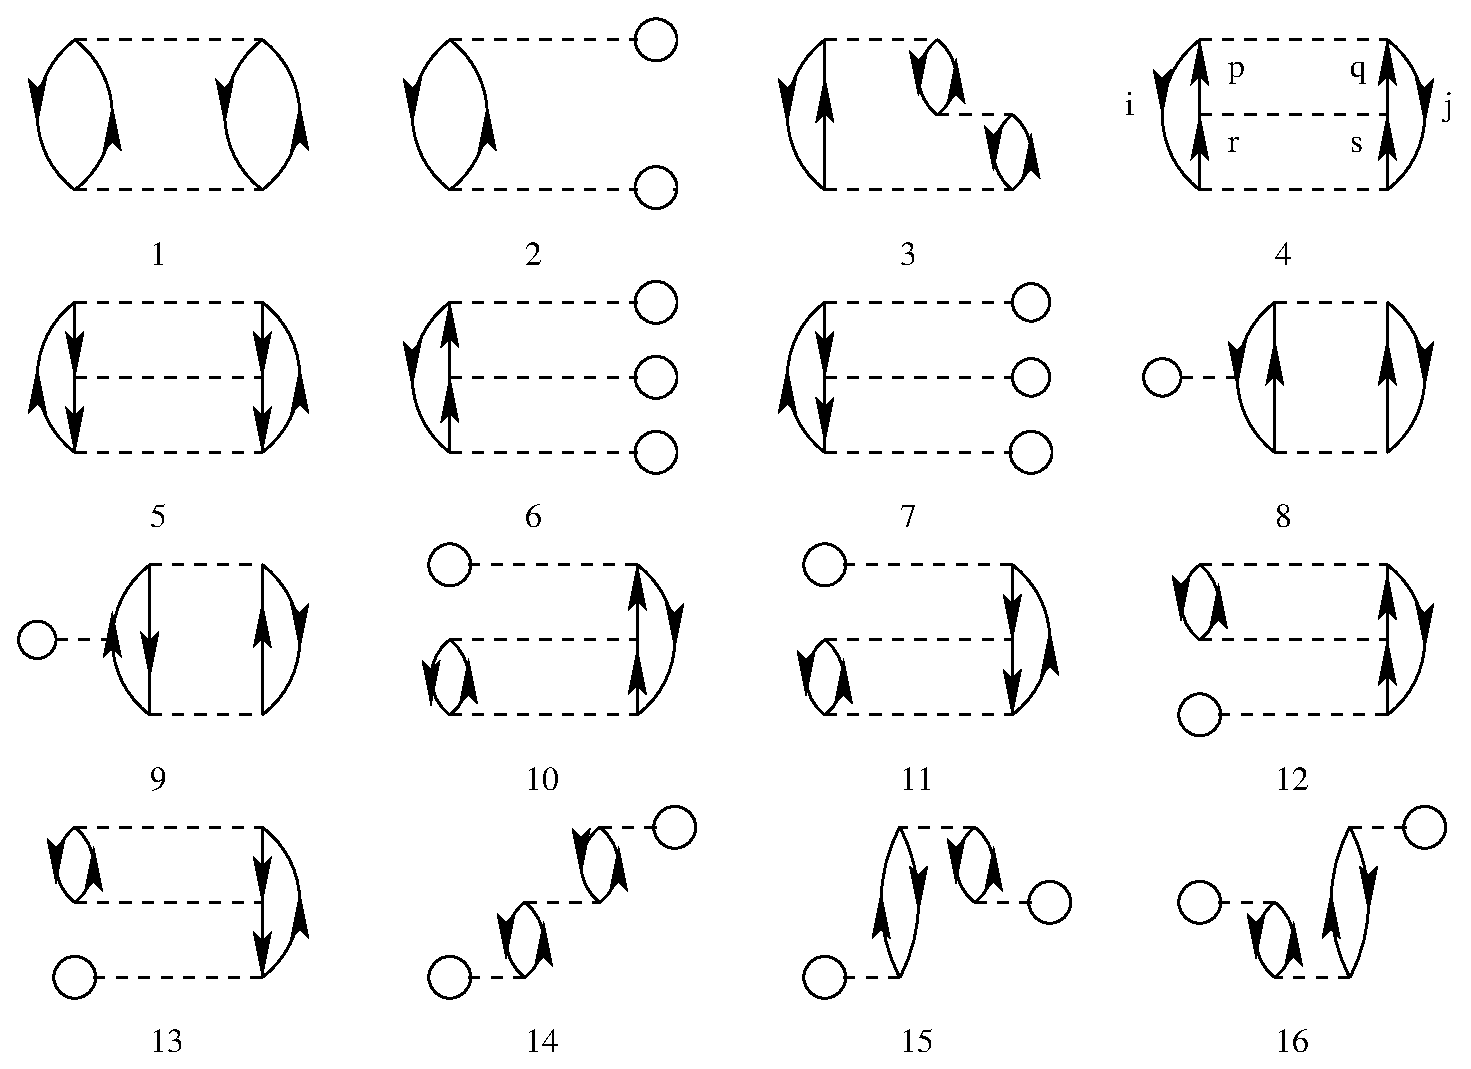
\includegraphics[width=.6\textwidth]{figures/diagrams.eps}
\caption{Diagrams to third order in the interaction. The first order
  term is excluded. All interaction vertices represent anti-symmetrized matrix elements.\label{fig:diagrams}}
\end{figure}

Based on the form of the interaction, which diagrams contribute to the
energy of the ground state?  Write down the expressions for
the diagrams that contribute and find the contribution to the ground
state energy as function $g\in [-1,1]$. Comment your results.  Compare
these results with those you obtained in 2) and 3).


\item  (10/100 points) Diagram 1 in Fig.~\ref{fig:diagrams} represents a second-order contribution to the energy and a so-called $2p-2h$ contribution to the intermediate states. Write down the expression for the wave operator in this case and compare the possible contributions with the configuration interaction calculations of exercise 3). Comment your results for 
various values of $g\in [-1,1]$.  
\item  (25/100 points) We limit now the discussion to the Hartree-Fock basis  we discussed above. To fourth order in perturbation theory we can produce diagrams with $1p-1h$ intermediate excitations as shown in Fig.~\ref{fig:fourthorder1p1h}, $2p-2h$ excitations, see Fig.~\ref{fig:fourthorder2p2h}, $3p-3h$ excitations as shown in Fig.~\ref{fig:fourthorder3p3h} and finally so-called diagrams with intermediate four-particle-four-hole excitations, see Fig.~\ref{fig:fourthorder4p4h}. 
\begin{figure}[hbtp]
\includegraphics{figures/1p1h.ps}
\caption{One-particle-one-hole excitations to fourth order.}
\label{fig:fourthorder1p1h}
\end{figure}
\begin{figure}[hbtp]
\includegraphics{figures/2p2h.ps}
\caption{Two-particle-two-hole excitations to fourth order.}
\label{fig:fourthorder2p2h}
\end{figure}
\begin{figure}[hbtp]
\includegraphics{figures/3p3h.ps}
\caption{Three-particle-three-hole excitations to fourth order.}
\label{fig:fourthorder3p3h}
\end{figure}
\begin{figure}[hbtp]
\includegraphics{figures/4p4h.ps}
\caption{Four-particle-four-hole excitations to fourth order.}
\label{fig:fourthorder4p4h}
\end{figure}


Based on the linked diagram theorem and the form of the pairing Hamiltonian, which diagrams will contribute
to fourth order?  Here we recommend reading Shavitt and Bartlett's chapter 4-6, and chapter 6 in particular about the linked diagram theorem.

Calculate the energy to fourth order with the Hartree-Fock basis defined earlier for $g\in [-1,1]$ and compare
with the full diagonalization case in exercise 2). Discuss the results.
\end{enumerate}



 \end{document}




